\clearpage
\subsection{Verificación de C3 revisión 02}
\label{sec:c3r02-resultados}
La revisión ampliada reduce la demanda total de enfriamiento de 84.759,41 a 65.767,88 kWh térmicos/año: una diferencia de 18.991,53 kWh y una reducción del 22,41\,\% respecto al caso base. Frente a C3 revisión 01, disminuye 16.981,08 kWh térmicos/año adicionales. El resultado corresponde al paquete conjunto de envolvente e iluminación; no permite atribuir el ahorro a un componente aislado.
\begin{table}[H]\centering
\caption{Resultado anual de la propuesta ampliada}
{\small\singlespacing\renewcommand{\arraystretch}{1.3}
\begin{tabular}{lrr}\toprule
Caso & Enfriamiento (kWh térmicos/año) & Reducción frente al CB (\%) \\ \midrule
Caso base & 84.759,41 & 0,00 \\
C3 revisión 01 & 82.748,96 & 2,37 \\
C3 revisión 02 & 65.767,88 & 22,41 \\
\bottomrule\end{tabular}}
\fuente{Elaboración propia con series horarias de EnergyPlus, calendario 2025 y clima común. Demanda térmica, no consumo eléctrico medido.}
\end{table}
La corrida finalizó con cero errores severos y 324 advertencias. Se amplió el máximo de días de inicialización de 25 a 100 para resolver la falta de convergencia inicial, conservando las tolerancias térmicas. La integración de 8.760 valores horarios coincide con el reporte anual, con diferencia inferior a 0,01 kWh. El cotejo con C3 revisión 01 confirma la conservación de geometría, clima, ocupación, equipos, horarios y consignas.

De los 19 controles de luz natural configurados, seis son ignorados por el motor porque sus zonas no tienen ventanas exteriores: PB-BO-01, PB-BA-01, PB-RE-01, 1PA-DC, 2PA-CAF y 2PA-PAS. La potencia de 8 W/m\textsuperscript{2} sí se aplica a las 19 zonas. El proyecto debe definir controles de presencia u otra solución apropiada para esos seis espacios y comprobar la cobertura exigida por E05. Las advertencias comunes de dimensionamiento y los supuestos del datacenter siguen siendo límites de la evaluación.

El 22,41\,\% cuantifica E01 frente al CB del proyecto. No acredita el umbral EDGE de E02, cuya referencia y balance de energía operacional requieren un cálculo específico. Tampoco demuestra por sí solo cumplimiento de confort ni certificación ambiental de los materiales.
\clearpage
\begin{figure}[H]\centering
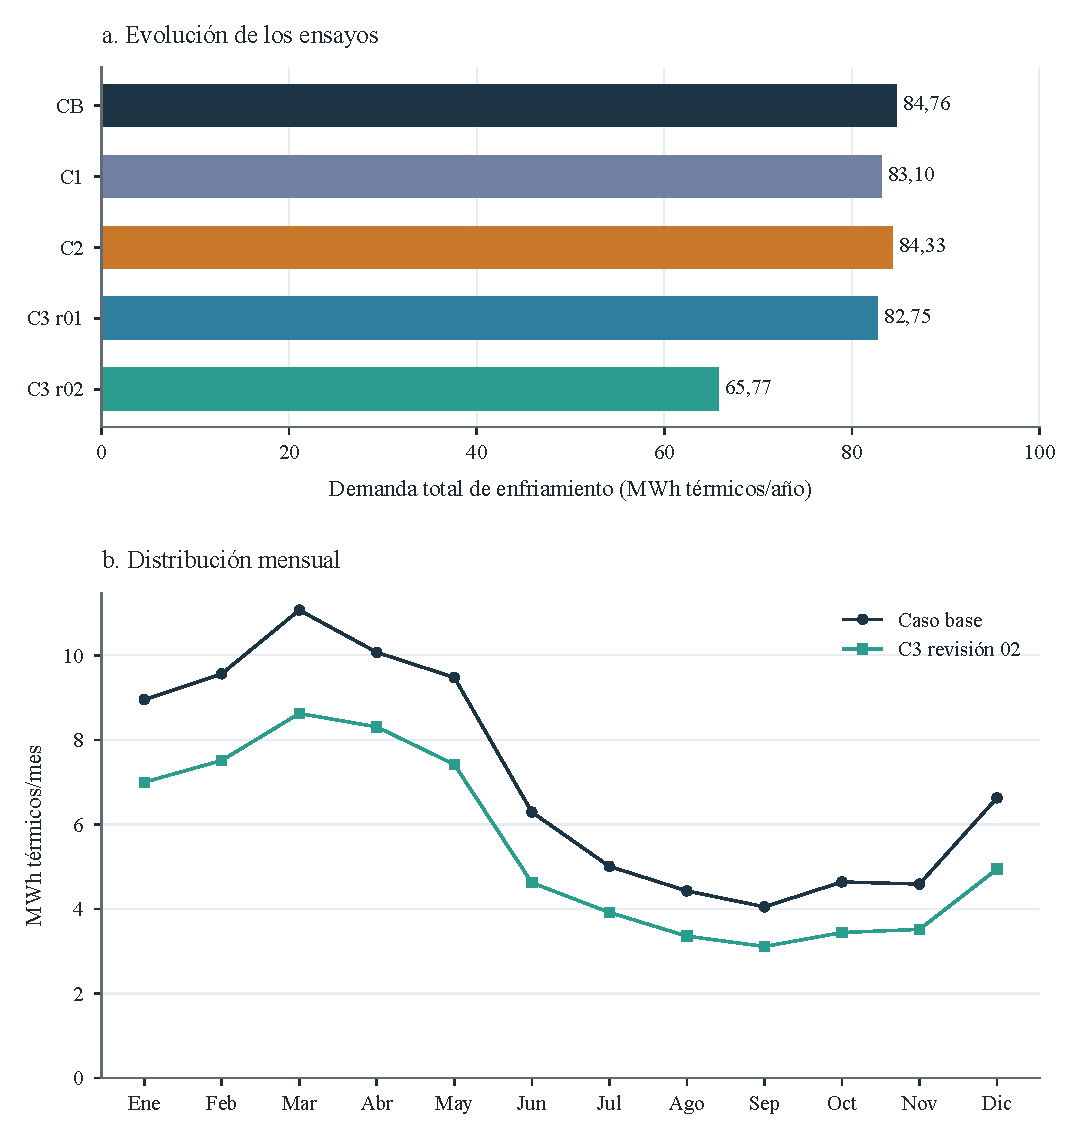
\includegraphics[width=0.94\textwidth]{figuras/escenarios/C3r02-comparacion.pdf}
\caption{Comparación anual de los ensayos y demanda mensual de la propuesta ampliada.}
\fuente{Elaboración propia con resultados de las cinco corridas. C3 r01 y C3 r02 son revisiones independientes; los colores identifican escenarios.}
\end{figure}
\clearpage
\begin{figure}[H]\centering
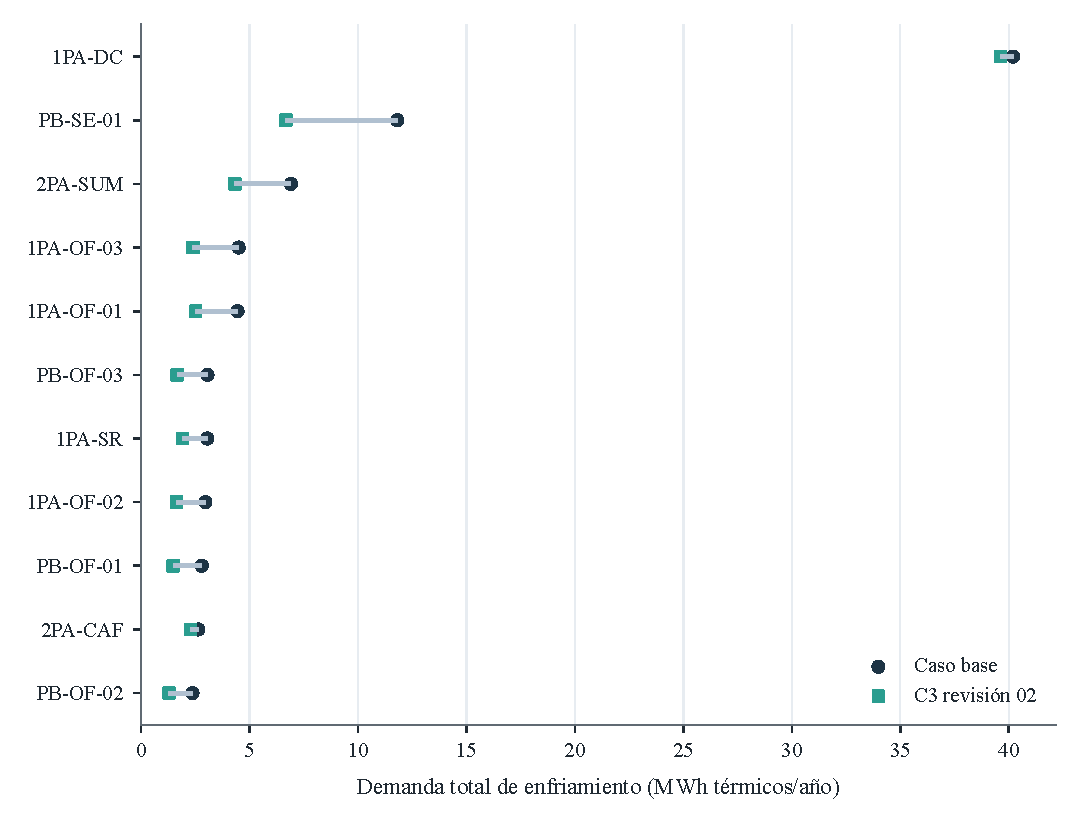
\includegraphics[width=\textwidth]{figuras/escenarios/C3r02-zonas.pdf}
\caption{Demanda anual de enfriamiento por zona: caso base y C3 revisión 02.}
\fuente{Elaboración propia. Se muestran las once zonas con demanda de enfriamiento distinta de cero en al menos uno de los dos modelos.}
\end{figure}
La comparación por zona permite localizar la respuesta del paquete y revisar los espacios con cargas internas persistentes. La permanencia de una demanda elevada no debe resolverse modificando arbitrariamente las cargas para obtener un porcentaje de ahorro mayor; requiere contrastar el uso y el equipamiento con el programa real del edificio.
